\chapter{Model equations}\label{chap:model_equations}

\section{How to navigate this chapter}

This chapter covers the fluid and associated field equations modelled by {\fluidity}.

\begin{center}
\begin{tabular}{lccc}
\hline
problem & underlying equations & boundary conditions & other considerations\\
\hline
scalar advection & \ref{sec:MP-AdvdifEqn-eqns}, \ref{sec:MP-AdvdifEqn-adv} & \ref{sec:bc_scalar_dirichlet}, \ref{sec:bc_scalar_neumann} & × \\
scalar advection-diffusion & \ref{sec:MP-AdvdifEqn-eqns}, \ref{sec:MP-AdvdifEqn-diff} & × & ×\\
momentum equation & \ref{sec:MP-MomEqn} & \ref{sec:bc_vector_dirichlet}, \ref{sec:bc_vector_stress}, \ref{sec:bc_vector_traction}, \ref{sec:FS} & \ref{sec:eqn_extensions} \\
\hline
\end{tabular}
\end{center}

The material covered in this chapter is dealt with in great detail in \citet{batchelor1967} and \citet{landau}. \cite{cushman1994} is also a useful reference.

\section{Advection--Diffusion equation}\label{sec:MP-AdvdifEqn}
\index{advection-diffusion equation}

\subsection{General equation}\label{sec:MP-AdvdifEqn-eqns}

The general form the equation that governs the evolution of a scalar field $c$
(\eg passive tracer, species concentration, temperature, salinity) is
\begin{equation}\label{eq:general_scalar_eqn}
\ppt{c} + \nabla\cdot(\bmu c) = \nabla\cdot(\kaptens\nabla c) - \sigma c + F,
\end{equation}
where $\bmu=(u,v,w)^{T}$ is the velocity vector, $\kaptens$ is the diffusivity (tensor), $\sigma$ is an absorption coefficient ($-\sigma c$ is sometimes termed Rayleigh or linear friction) and $F$ represents any source or reaction terms.

\subsubsection{Advection}\label{sec:MP-AdvdifEqn-adv}
The advection term in \eqref{eq:general_scalar_eqn}, given by
\begin{equation}\label{eq:scalar_advection}
\nabla\cdot(\bmu c) = \bmu\cdot\nabla c + (\nabla\cdot\bmu)c,
\end{equation}
expresses the transport of the scalar quantity $c$ in the flow field $\bmu$. Note that for an incompressible flow $\nabla\cdot\bmu=0$ (see section \ref{sec:equation_of_state}) resulting in the second term on the right hand side of \eqref{eq:scalar_advection} dropping out. However, there may be numerical
reasons why the discrete velocity field is not exactly divergence free, in which case this term may
be included in the discretisation. {\fluidity} deals with the advection term in the form
\begin{equation}\label{eq:fluidity_scalar_advection}
\nabla\cdot(\bmu c) + (\beta-1)(\nabla\cdot\bmu)c,
\end{equation}
so that $\beta=1$ corresponds to the conservative form of the equation and $\beta=0$ to the non-conservative.

\subsubsection{Diffusion}\label{sec:MP-AdvdifEqn-diff}
The diffusion term in \eqref{eq:general_scalar_eqn}, given by 
\begin{equation}\label{eq:scalar_diffusion}
\nabla\cdot(\kaptens\nabla c),
\end{equation}
represents the mixing of $c$ and may be due to 
molecular mixing of individual particles via Brownian motion, or mixing via large scale (in comparison to the
molecular scale) motion in the flow. For many applications \eqref{eq:scalar_diffusion} can be written in simpler forms. Often, diffusion is isotropic giving $\kaptens = \mathrm{diag}(\kappa,\kappa,\kappa)$ and thus the diffusion term
may be written as
\begin{equation}\label{eq:scalar_isotropic_diffusion}
\nabla\cdot(\kaptens\nabla c) = \kappa\nabla\cdot\nabla c = \kappa\nabla^2 c = \kappa\Delta c.
\end{equation}
In domains with high aspect ratio dynamics one often uses a smaller value of diffusivity in the `thin'
direction. For example, in the atmosphere or ocean we may choose a horizontal (eddy) diffusivity $\kappa_H$ and a
vertical (eddy) diffusivity $\kappa_V$ so that $\kaptens = \mathrm{diag}(\kappa_H,\kappa_H,\kappa_V)$ with $\kappa_V < \kappa_H$.
In this case the diffusion term may be written as
\begin{equation}\label{eq:scalar_anisotropic_diffusion}
\nabla\cdot(\kaptens\nabla c) = \kappa_H \left(\pptt[x]{c} + \pptt[y]{c}\right) + \kappa_V \pptt[z]{c}.
\end{equation}
Note that the second-order terms defined above are often termed Laplacian diffusion.


\subsubsection{Absorption, reaction and source terms}\label{sec:MP-AdvdifEqn-abs}
\index{absorption term}
\index{source term}
\index{reaction term}

The absorption term in \eqref{eq:general_scalar_eqn} 
\begin{equation}\label{eq:scalar_absorption}
-\sigma c,
\end{equation}
has the effect of decreasing the magnitude of $c$ (note the minus sign and the fact 
that $\sigma$ would typically be positive). It is sometimes termed Rayleigh friction. 

The remaining term in \eqref{eq:general_scalar_eqn}
\begin{equation}\label{eq:scalar_source}
F = \sum_i F_i,
\end{equation}
can encompasses a number of source and reaction terms. Those terms where $F_i$ are
a given function of time, location or a-priori known fields are termed sources (and sometime
sinks if they are negative). Those terms which are also functions of other prognostic fields
are termed reactions and are common when dealing with chemistry or biology.

\subsection{Scalar boundary conditions} \label{sec:BCs}

\index{boundary conditions!scalar}

To form a well-posed system upon which to attempt a numerical discretisation, the
set of equations (discussed above) describing the behaviour of the 
system must be supplemented with appropriate boundary conditions.


\subsubsection{Dirichlet condition for a scalar field}\label{sec:bc_scalar_dirichlet}
\index{boundary conditions!Dirichlet}
For a scalar field, $c$ say, a Dirichlet condition on the boundary
$\partial\Omega$ takes the form
\begin{equation*}
c=\tilde{c},\quad \textrm{on}\quad \partial\Omega.
\end{equation*}


\subsubsection{Neumann condition for a scalar field}\label{sec:bc_scalar_neumann}
\index{boundary conditions!Neumann}

Taking the weak form (applying Green's theorem to the diffusion term) of the advection-diffusion equation \eqref{eq:general_scalar_eqn} leads to a surface integral of the form
\begin{equation*}
\int_{\partial\Omega} \phi (\kaptens\nabla c)\cdot\bmn \;d\Gamma,
\end{equation*}
where $\phi$ is a test function (see section \ref{chap:numerical_discretisation}).
The Neumann condition is specified by assigning a value to $(\kaptens\nabla c)\cdot\bmn$, \eg
\begin{equation*}
(\kaptens\nabla c)\cdot\bmn = q,\quad \textrm{on}\quad \partial\Omega,
\end{equation*}
and substituting in this surface integral to the discretised equation. Note that $q$ is often termed a flux.


\section{Fluid equations}\label{sec:MP-MomEqn}

\index{conservation!equation}
\index{momentum equation}

A starting point for describing the physics of a continuum are the conservation equations. Fluid volumes deform in time as the fluid moves. If $\theta(\bmx,t)$ is the density of some quantity (\eg Temperature) associated with the fluid, the time evolution of that quantity in a fluid volume $V(t)$ is 
\begin{equation}\label{RTT}
 \ddt{}\left[\int_{V(t)}\theta(\bmx,t)\right]=
 \int_{V(t)}\left(\DDt{\theta}+\theta\nabla\cdot\bmu\right),
\end{equation}
which is the Reynolds' Transport theorem. In \eqref{RTT} $\bmx=(x,y,z)^T$ and $\bmu=(u,v,w)^T$ are three-dimensional position and velocity vectors respectively and 
\begin{equation}\label{MatDiv}
 \DDt{}\equiv\frac{\partial}{\partial{t}}+\bmu\cdot\nabla,
\end{equation}
is the \textit{material derivative} (NB. it has many other commonly-used names including the total and Lagrangian derivative). \index{Reynolds Transport theorem}

\subsection{Mass conservation}
\index{conservation!mass}
Substituting $\theta=\rho$ in to \eqref{RTT} and noting that matter is neither created nor destroyed gives that the \lhs\ of \eqref{RTT} is zero. Then, as the volume $V(t)$ is arbitrary, it is seen that the mass density satisfies
\begin{equation}\label{mass_conservation}
 \DDt{\rho}=-\rho\nabla\cdot\bmu,
\end{equation}
or equivalently
\begin{equation}\label{mass_conservation_2}
 \frac{\partial\rho}{\partial{t}}+\nabla\cdot(\rho\bmu)=0.
\end{equation}
The quantity $\rho\bmu$ is called the \textit{mass flux} or \textit{momentum} and \eqref{mass_conservation_2} is termed the \textit{equation of continuity}.

\subsection{Momentum conservation}
\index{conservation!momentum}
The momentum associated with a unit volume of fluid is given by $\rho\bmu$. Initially, consider that the fluid is \textit{ideal}, that is, viscosity and conductivity are assumed to be unimportant. Then, the rate of change of momentum is given by
\begin{equation}\label{mom_cons_1}
 \frac{\partial}{\partial{t}}(\rho\bmu)=\rho\frac{\partial\bmu}{\partial{t}}+\frac{\partial\rho}{\partial{t}}\bmu.
\end{equation}
Using the equation of continuity \eqref{mass_conservation_2} and Euler's
equation \citep{batchelor1967} (the force equation for an inviscid fluid) in the form
\begin{equation}\label{mom_cons_2}
 \frac{\partial\bmu}{\partial{t}}=-\bmu\cdot\nabla\bmu-\frac{1}{\rho}\nabla{p},
\end{equation}
gives
\begin{equation}\label{mom_cons_3}
 \frac{\partial}{\partial{t}}(\rho\bmu)=-\nabla{p}-\nabla\cdot(\rho\bmu\bmu),
\end{equation}
where $\bmu\bmu$ is a tensor which represents the dyadic product of vectors which, using index notation, can be written as ${u_{i}u_{j}}$. Writing $\tensor{\Pi}=p\mathbf{I}+\rho\bmu\bmu$, \eqref{mom_cons_3} can be written as
\begin{equation}\label{mom_cons_4}
 \frac{\partial}{\partial{t}}(\rho\bmu)+\nabla\cdot\tensor{\Pi}=0,
\end{equation}
where $\tensor{\Pi}$ is clearly a symmetric tensor and is termed the \textit{momentum flux density tensor}.

The effects of viscosity on the motion of a fluid are now considered. To express the equations of motion governing a viscous fluid, some additional terms are required. The equation of continuity (conservation of mass) is equally valid for any viscous as well as inviscid fluid. However, Euler's equation \eqref{mom_cons_2} and hence \eqref{mom_cons_4} require modification.

By adding $-\tautens$ to the previously introduced \textit{momentum flux density tensor}, $\tensor{\Pi}$, so that

\begin{equation}
 \tensor{\Pi}=p\mathbf{I}+\rho\bmu\bmu-\tautens=-\sigtens+\rho\bmu\bmu,
\end{equation}

where $\sigtens=-p\mathbf{I}+\tautens$, the viscous transfer of momentum in the fluid can be taken into account. $\sigtens$ is called the stress tensor and gives the part of the momentum flux which is not due to direct transfer of momentum with the mass of the fluid. $\tautens$ is named the deviatoric or viscous stress tensor. These tensors and the forms which they may take are discussed in more detail in section \ref{sec:equation_of_state}. Thus, the most general form of the momentum equation of a compressible viscous fluid may be written as

\begin{equation}\label{viscous_fluids_1}
 \rho\left(\frac{\partial\bmu}{\partial{t}}+\bmu\cdot\nabla\bmu\right)=-\nabla\cdot\sigtens+\rho\bmF,
\end{equation}

where $\bmF$ is a volume force per unit mass (\eg gravity, astronomical forcing).

% Note: Something needs to be added about the difference between the two forms outlined below within Fluidity i.e. a reference
% to somewhere in chapter 3 that goes over this.

\subsubsection{Compressible equations in conservative form}\label{sec:compressible_conservative}
Using the conservation laws outlined above the following point-wise PDE system governing the motion of a compressible fluid is obtained

\begin{subeqnarray}
\frac{\pp\rho}{\pp t} + \nabla\cdot(\rho\bmu) &=& 0,\slabel{conmass}\\
\frac{\pp}{\pp t}(\rho\bmu) + \nabla\cdot(\rho\bmu\bmu-\sigtens) &=& \rho\bmF,\slabel{conmom}\\
\frac{\pp}{\pp t}(\rho \tote) + \nabla\cdot(\rho E\bmu - \sigtens\bmu +
\bmq) &=& \rho\bmF\cdot\bmu,\slabel{conenergy}
\label{conservativesystem}
\end{subeqnarray}
where $\tote\equiv\inte+\modu^2/2$ is the total specific energy (in which $\inte$ is the internal energy). \eqref{conmass} is exactly the conservative form of the continuity equation given in \eqref{mass_conservation_2}, \eqref{conmom} is equivalent to equation \eqref{viscous_fluids_1} and \eqref{conenergy} is obtained from making the substitutions $w=\inte+p/\rho$ and $\tote\equiv\inte+\modu^2/2$ in \eqref{viscous_fluids_1}.

\subsubsection{Compressible equations in non-conservative form}\label{sec:compressible_nonconservative}
Expanding terms in \eqref{conservativesystem} yields the
non-conservative form of the compressible equations\footnote{\eqref{nonconmass}
is trivial to obtain. \eqref{nonconmom} makes use of \eqref{conmass}
and the divergence of the dyadic product, given by
\begin{equation*}
\nabla\cdot(\bmu\bmu) = \bmu\cdot\nabla\bmu + \bmu\nabla\cdot\bmu,
\end{equation*}
along with \eqref{MatDiv}. \eqref{nonconenergy} makes use of both \eqref{nonconmass} and \eqref{nonconmom} and
note that substituting for $\tote\equiv\inte+\modu^2/2$ results in the cancellation of kinetic energy terms.}
\begin{subeqnarray}\label{nonconform}
\DDt{\rho} + \rho\nabla\cdot\bmu &=& 0,\slabel{nonconmass}\\
\rho\DDt{\bmu} -\nabla\cdot\sigtens &=& \rho\bmF,\slabel{nonconmom}\\
\rho\DDt{\inte} - \sigtens\cdot\nabla\bmu + \nabla\cdot\bmq &=&
0.\slabel{nonconenergy} \label{nonconservativesystem}
\end{subeqnarray}
Note that, provided the fields (\eg density and pressure) vary smoothly, that is, the fields are differentiable functions, equations \eqref{conservativesystem} and \eqref{nonconservativesystem} are identical.

\subsection{Equations of state \& constitutive relations}
\label{sec:equation_of_state}
\index{equation of state}

Closure of the conservation equations requires an additional equation describing how the stress tensor is related to density, temperature and any other state variables of relevance. In general, this relationship is dependent of the physical and chemical properties of the material in the domain; hence, this relationship is known as the material model (note that in multi-material simulations a different material model can and must be specified for each material).

It is convenient to separate the full stress tensor $\sigtens$ into an isotropic (hydrostatic) part, the pressure $p$, and a deviatoric part $\tautens$.  With the convention that compressive stress is negative, the stress tensor is given by $\sigtens =-p \bmI + \tautens$, where $\bmI$ is the identity matrix. If the stress tensor is separated in this way, the material model comprises two parts: an equation of state\footnote{Equation of state settings in \fluidity\ are described in section~\ref{sec:ConfigEOS}} $f(p,\rho,T,\ldots)=0$ relating density to pressure, temperature, etc., and a constitutive relationship\footnote{constitutive relationship settings in \fluidity\ are described in section (to be written)} $g(\tautens,\bmu)=0$.

\subsubsection{Newtonian fluids}
\index{stress}
\index{strain}

Two important classes of fluids are: (i) Newtonian fluids, where deviatoric strain rate $\left(\etens\right)$ is linearly proportional to deviatoric stress ($\tautens$); and (ii) non-Newtonian fluids, where deviatoric strain rate is non-linearly proportional to the deviatoric stress. At present \fluidity\ is only configured to deal with Newtonian fluids.

For a Newtonian fluid the relation between deviatoric stress and deviatoric strain rate can be expressed as: 

\begin{equation}
\tautens = 2\mu \etens + \lambda(\nabla\cdot\bmu)\bmI,
\end{equation}
where 
\begin{equation}
 \etens = \frac{1}{2}(\nabla\bmu + (\nabla\bmu)^T),
\end{equation}
is the
deviatoric strain rate tensor, and $\bmI$ is the identity matrix. $\mu$ and
$\lambda$ are the two coefficients of viscosity. Physical arguments
yield the so-called Stokes' relationship $3\lambda+2\mu=0$, and
hence:
\begin{equation}
\tautens = 2\mu(\etens - (\nabla\cdot\bmu)\bmI/3),
\end{equation}
where $\mu$ is the molecular viscosity. See \cite{batchelor1967} for further
details.

\subsubsection{Equation of state for incompressible flow}
\label{sec:IncompressibleFlow}
\index{equation of state}

If a material is \emph{perfectly} incompressible its density cannot change;
in other words, the material density is independent of pressure and
temperature, giving $\rho = \rho_0$, where $\rho_0$ is the reference
density. Note that a flow may contain multiple incompressible materials of
different densities, in which case $\rho^k=\rho_0^k$ applies for each
individual material (indexed with the superscript $k$).

All real materials are compressible to some extent so that changes in
pressure and temperature cause changes in density.  However, in many
physical circumstances such changes in material density are sufficiently
small that the assumption of incompressible flow is still valid. If $U/L$ is
the order of magnitude of the spatial variation in the velocity field, then
the flow field can be considered incompressible if the relative rate of
change of density with time is much less than the spatial variation in
velocity; \ie if $\frac{1}{\rho}\DDt{\rho}\ll U/L$ then \cite[][p.167]{batchelor1967}.

\begin{equation}\label{eq:divfree}
\nabla\cdot\mathbf{u}\approx 0.
\end{equation}

The term incompressible flow is used to describe any such situation where
changes in the density of a parcel of material are negligible.  Not all
parcels in the flow need have the same density; the only requirement is that
the density of each parcel remains unchanged.  For example, in the ocean
where salt content and temperature change with depth, the density of
adjacent parcels changes but any one parcel has a constant density
\cite{panton2006}.  In such cases it is often important to account for
changes in buoyancy caused by the dependence of density on pressure,
temperature and composition $C$ (see, for example,
section~\ref{sec:boussinesq_approximation}).  If the change in $\rho,p,T,C$
about a reference state $\rho_0,p_0,T_0,C_0$ is small, the dependence of
density on each state variable can be assumed to be linear.  In this case, a
general equation of state takes the form
\index{equation of state!linear}
\begin{equation}
\rho = \rho_0(1 - \alpha(T-T_0) + \beta(C-C_0) + \gamma(p-p_0)),
\end{equation}
where $\alpha$ is the thermal expansion coefficient:
\begin{equation*}
\alpha = -\frac{1}{\rho}\frac{\pp\rho}{\pp T},
\end{equation*}
$\beta$ is a general compositional contraction coefficient
\begin{equation}
\beta = \frac{1}{\rho}\frac{\pp\rho}{\pp C},
\end{equation}
and $\gamma$ is the isothermal compressibility
\begin{equation}
\gamma = \frac{1}{\rho}\frac{\pp\rho}{\pp p}.
\end{equation}

For ocean modelling applications the most important compositional variation is salinity $S$ (the volume fraction of salt) and the compressibility of water $\gamma$ is so small that the pressure dependence can be neglected, giving the simple linear equation of state
\begin{equation}
\rho = \rho_0(1 - \alpha(T-T_0) + \beta(S-S_0)),
\end{equation}
where $\beta$ is the saline contraction coefficient (not to be confused with the beta plane parameters defined in the section \ref{sec:coriolis}.)

\subsubsection{Pade equation of state for ocean modelling}\label{sec:PadeDescription}
\index{equation of state!Pade approximation}

Within \fluidity it is also possible to relate the density of sea water to the in situ temperature and salinity through the Pad{\'e} approximation to the equation of state. This approximation offers an accurate and computationally efficient method for calculating the density of seawater and is described by \citet{mcdougall2003}.

% The Pade approx may not actually be coded for the in situ temp, this needs to be checked.

\subsection{Momentum boundary conditions} \label{sec:BCs-mom}

\index{boundary conditions!Momentum}

As with the scalar equations discussed previously in section \ref{sec:MP-AdvdifEqn}, any well posed problem requires appropriate boundary conditions for the momentum equation. Possible momentum boundary conditions are discussed below.

\subsubsection{Prescribed Dirichlet condition for momentum --- no-slip as a special case}\label{sec:bc_vector_dirichlet}
\index{boundary conditions!Dirichlet}
\index{momentum equation}

This condition for momentum is set by simply prescribing all three components of
velocity. For example, we might specify an inflow boundary where the normal component
of velocity is non-zero, but the two tangential directions are zero. A special case is
where all three components are zero and this is referred to as no-slip.

\subsubsection{Prescribed stress condition for momentum --- free-stress as a special case}\label{sec:bc_vector_stress}
\index{boundary conditions!prescribed stress}
\index{traction force}
\index{momentum equation}

As with the scalar equation (see section \ref{sec:bc_scalar_neumann}), applying Green's theorem to the stress term and the pressure
gradient in \eqref{mtm} results in a surface integral of the form
\begin{equation}\label{StressBC}
\tautens\cdot\bmn - p\bmn = \bmT,\quad \textrm{on}\quad \partial\Omega,
\end{equation}
where $\bmT$ is an applied `traction' force (actually a force per unit area or stress, it becomes
a force when the surface integral in the weak form is performed). An example of this might be were we set the vertical
component to zero (in the presence of a free surface) and impose the two tangential directions
(\eg a wind stress).

\index{boundary conditions!free stress}
The free-stress condition is the case where we take $\bmT\equiv\vec{0}$.

\subsubsection{Traction boundary condition for momentum --- free-stress as a special case}\label{sec:bc_vector_traction}
\index{boundary conditions!traction}
\index{momentum equation}
In this case the normal component of velocity can be prescribed (\eg inflow or
no-flow ($g=0$) through the boundary)
\begin{equation*}
\bmu\cdot\bmn = g,\quad \textrm{on}\quad \partial\Omega.
\end{equation*}
The remaining two degrees of freedom are imposed by taking the
tangential component of \eqref{StressBC} and specifying the tangential component
of the force $\bmT_{\tau}$, \ie
\begin{equation*}
\bmtau\cdot(\tautens\cdot\bmn - p\bmn) = \bmtau\cdot\tautens\cdot\bmn = \bmT_{\tau},\quad \textrm{on}\quad \partial\Omega,
\end{equation*}
An example of this might be where a rigid lid is used (so normal component is zero)
and the tangential components are a prescribed wind stress (in which case we take
the two tangential directions to correspond to the available stress or wind velocity
information, \ie east-west and north-south) or bottom drag. Also, what we often term free-slip
where the tangential components of stress are set to zero.

\subsubsection{Free surface boundary condition}\label{sec:FS}
\index{free surface}
The free surface height $\eta\equiv\eta(x,y,t)$ measured from the initial state of the ocean
may be modelled either via the integrated continuity equation,
or for simplicity here by the kinematic boundary condition which simply states
that particles on the free surface remain on it, \ie
\begin{equation}\label{freesurf2}
\frac{\partial \eta}{\partial t}=-\left.{\bmu}_H\right|_{z=\eta}\cdot\nabla_H \eta +\left.w\right|_{z=\eta} \quad \textrm{on}\quad \Omega_{FS},
\end{equation}
where $\Omega_{FS}\subset \partial \Omega$ is the free surface boundary, $\nabla_H\equiv(\partial/\partial x,\partial/\partial y)^T$, and
$\bmu_H$ is the horizontal component of $\bmu$. Using the fact that the normal vector $\vec n$ at the free surface is $\frac{(-\frac{\partial \eta}{\partial x},-\frac{\partial \eta}{\partial y}, 1)^T}{||(-\frac{\partial \eta}{\partial x},-\frac{\partial \eta}{\partial y}, 1)^T||}$, equation \eqref{freesurf2} can be reformulated to
\begin{equation}\label{freesurf3}
\frac{\partial \eta}{\partial t}=\frac{\bmu \cdot \vec n}{\vec n \cdot \vec k},
\end{equation}
where $\vec k=(0,0,1)$ is the vertical standard basis vector. Note that in spherical geometries $\vec k$ is replaced with
$\vec r=(\sin\theta\cos\phi,\sin\theta\sin\phi,\cos\theta)$ where $\phi$ and $\theta$ are the azimuthal and co-latitudinal angles respectively. 

\subsubsection{Wetting and drying}\label{sec:WD}
\index{free surface!Wetting and drying}
If wetting and drying occurs, the free surface boundary condition \ref{freesurf3} needs to be changed to ensure that the water level $\eta$ does not sink below the bathymetry level $b$:

\begin{equation}\label{eq:wd1}
\frac{\partial \max(\eta, b+d_0)}{\partial t}=\frac{\bmu \cdot \vec n}{\vec n \cdot \vec k},
\end{equation}
where $d_0$ is a threshold defining the minimum water depth.

The details of the wetting and drying are described in \cite{Funke2011}.

\section{Extensions, assumptions and derived equation sets}\label{sec:eqn_extensions}

In certain scenarios it is desirable to simplify the equations of sections \ref{sec:MP-AdvdifEqn} and \ref {sec:MP-MomEqn} according to various approximations. Such approximations can drastically reduce the complexity of the system under consideration while maintaining much of the important physics. In this section we consider approximate forms and assumptions of the conservation equations that are appropriate to different problems. 

\subsection{Equations in a moving reference frame}\label{sec:coriolis}
\index{Coriolis}
Newton's second law holds in a fixed inertial reference frame, \ie
fixed with respect to the distant stars. 
Examples of systems which one may wish to study with boundaries moving
with respect to this fixed inertial frame include translating and spinning tanks
and the rotating Earth. For these systems it is often convenient to rewrite the 
underlying equations within the moving frame. Extra terms then need to be considered 
which account for the fact that the acceleration of a fluid parcel relative to the 
moving reference frame is different to the acceleration with respect to the fixed 
inertial frame, and the latter is the one which allows us to invoke Newton's Laws.
For useful discussions see \citep{batchelor1967,cushman1994,gill1982}.

\begin{figure}\label{fig:rotating_frame}
\centering
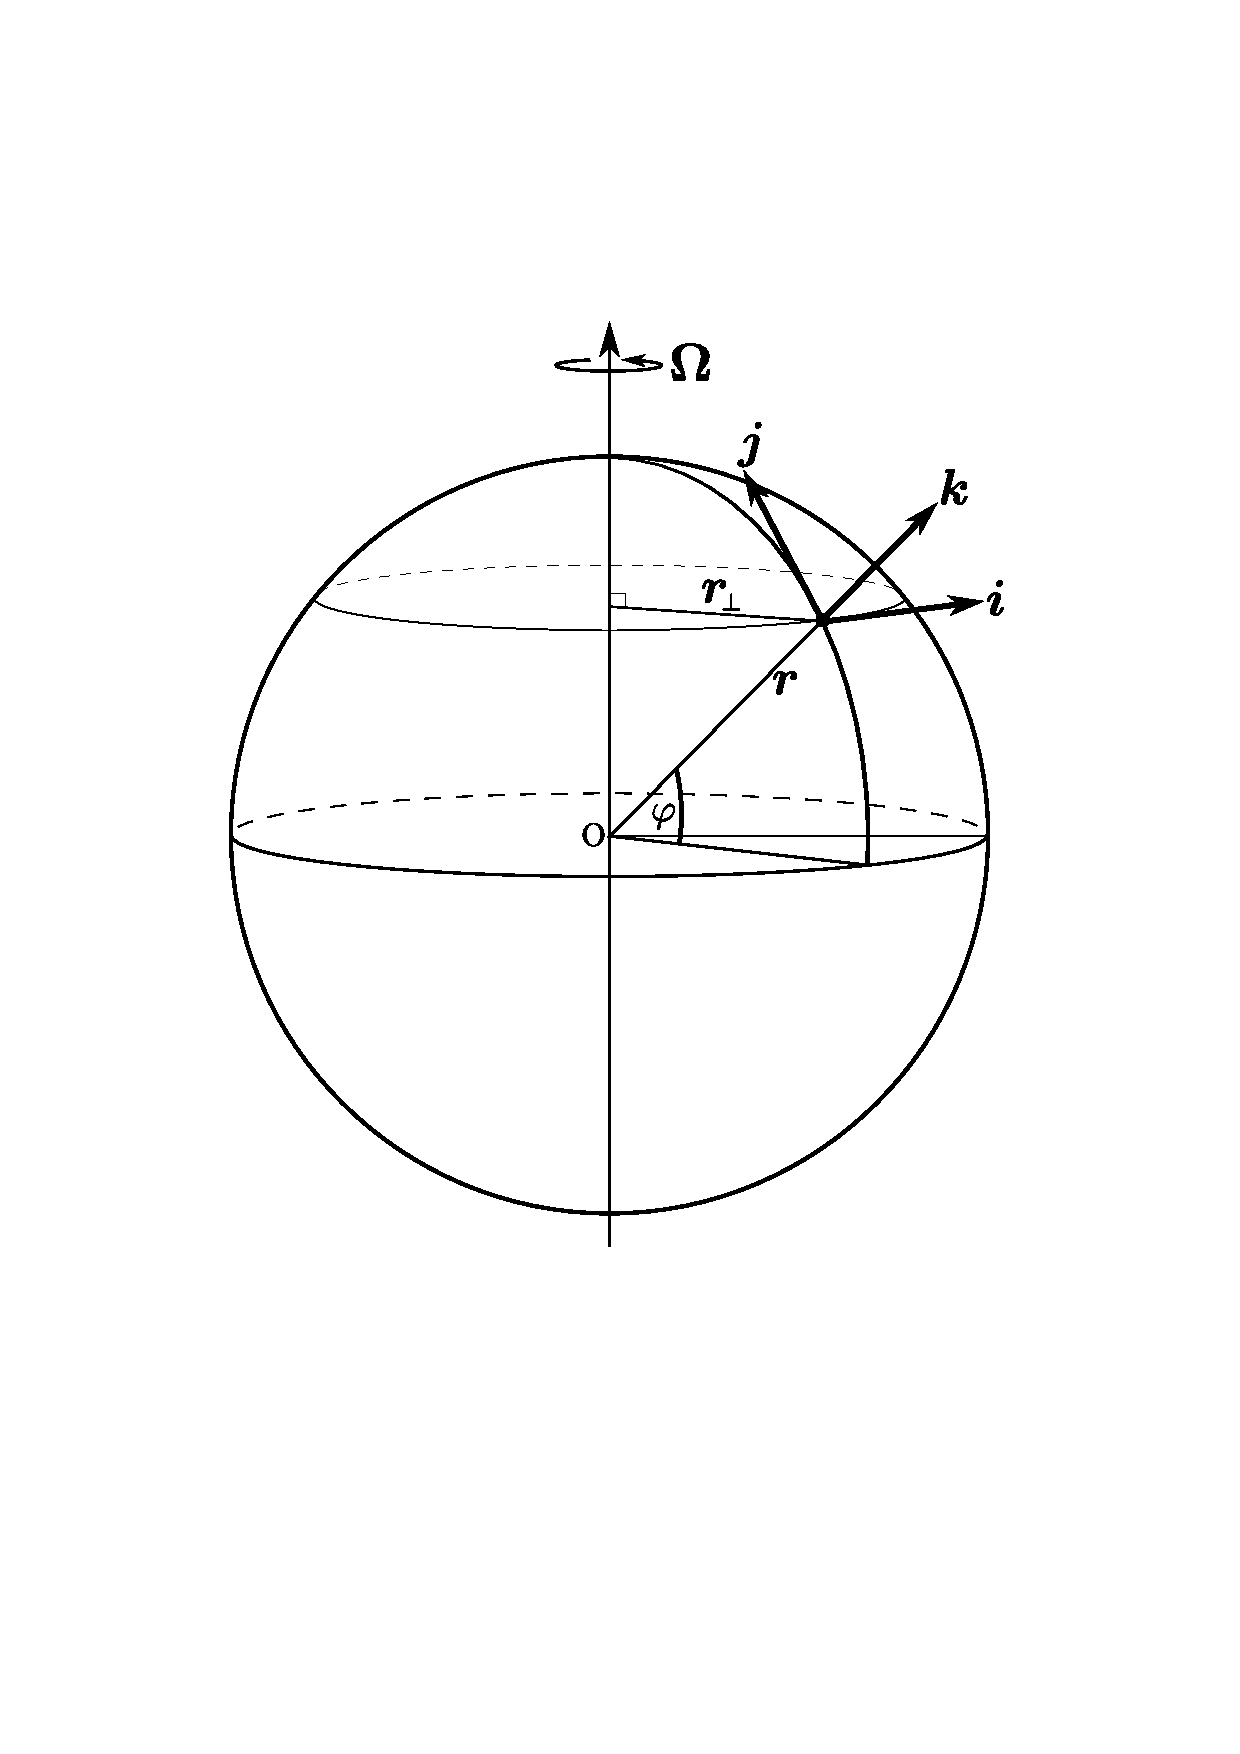
\includegraphics[width=8.0cm]{misc_images/coordinates.pdf}
\caption{Schematic of coordinates in a frame rotating with a sphere. The rotation is about a vector
pointing from South to North pole. A point on the surface of the sphere $\bmx$ and its perpendicular
distance from the axes of rotation $\bmx_{\perp}$ are shown. The latitude of $\bmx$ is given by $\phi$ 
and the unit vectors $\bmi$, $\bmj$ and $\bmk$ represent a local coordinate axes at a point $\bmx$ in the rotating
frame: $\bmi$ points Eastwards, $\bmj$ points Northwards and $\bmk$ points in the radial outwards direction.}
\end{figure}

It is possible to form the equations with respect to a moving reference frame as long as the
additional force or acceleration term is included. In the case of a rotating frame that is
just by replacing the material derivative in the momentum equation by
\begin{equation}
\DDt{\bmu} + 2\bmOmega\times\bmu,
\end{equation}
where $\bmOmega$ is the angular velocity vector of the rotating
system.

Consider the Earth with a rotation vector in an inertial reference frame given by 
\begin{equation}\label{eq:on_sphere_rotation}
\bmOmega=(0,0,\Omega)^T.
\end{equation}
In a local rotating frame of reference where the
$x$-axis is oriented Eastwards,
the $y$-axis is oriented Northwards and the $z$-axis is the local upwards direction,
the Earth's rotation vector is expressed as
\begin{equation*}
\bmOmega = \Omega \cos \phi\; {\bf j} + \Omega \sin \phi\; {\bf k} \equiv \Omega (0,\cos\phi,\sin\phi)^T,
\end{equation*}
where $\phi$ is the latitude.
The acceleration terms in the three momentum equations now have the form
{\setlength\arraycolsep{2pt}
\begin{eqnarray*}
&&\DDt{u} {\color{red}+} {\color{red}2\Omega\cos\phi\; w} - 2\Omega\sin\phi\; v,\\
&&\DDt{v} + 2\Omega\sin\phi\; u,\\
&&\DDt{w} {\color{red}-} {\color{red}2\Omega\cos\phi\; v}.
\end{eqnarray*}}

\subsubsection{The `traditional' approximation}
\index{traditional approximation}
Define the Coriolis and reciprocal Coriolis parameters \citep{cushman1994} respectively by
\begin{equation}\label{eq:coriolis_parameters} 
f=2\Omega\sin\phi,\quad f^*=2\Omega\cos\phi.
\end{equation}
Due to dimensional considerations it is is usual to
drop the $f^*$ term and hence simply assume that 
\begin{equation}\label{eq:f_omega}
\bmOmega=(0,0,f/2)^T,
\end{equation}
in the local frame of reference, \ie only to consider the locally vertical
component of the rotation vector.
This approximation, when taken along with the assumption of hydrostatic balance in the
vertical constitutes what is generally known as the traditional approximation in geophysical fluid
dynamics.


\subsubsection{The $f$-plane and $\beta$-plane approximations}
\index{Coriolis!f-plane@$f$-plane}
\index{Coriolis!b-plane@$\beta$-plane}
If the Coriolis parameter $f$ is approximated by a constant value:
\begin{equation}\label{eq:f-plane}
f=f_0,
\end{equation}
this is termed the $f$-plane approximation, 
where $f_0 = 2\Omega\sin\phi_0$ at a latitude $\phi_0$.
This is obviously only an applicable approximation in a domain of interest 
that does not have large extent in latitude. 

For slightly larger domains a more accurate approximation is to use
\begin{equation}\label{eq:beta-plane}
f = f_0 + \beta y,
\end{equation}
where $y$ is the local coordinate in the Northwards direction.
Taking $\phi = \phi_0 + y/R_E$ and expanding \eqref{eq:coriolis_parameters} 
in a Taylor series yields
\begin{equation*}
f = f_0 +2\Omega\cos\phi_0\frac{y}{R_E}+\ldots,\quad \beta = \frac{2\Omega}{R_E}\cos\phi_0,
\end{equation*}
where $R_E\approx\unit[6378]{km}$. Typical values of these terms are: 
\begin{equation*}
\Omega = \frac{2\pi}{24\times 60\times 60} = 7.2722\times 10^{-5}\rads[],
\end{equation*}
(NB. a sidereal day should be used to give a more accurate value of $7.2921\times 10^{-5}\rads[]$)
and
\begin{center}\begin{small}
\begin{tabular}{c|ccc}
  &  $\phi_0 = 30$ & $\phi_0=45$ & $\phi_0 = 60$ \\  \hline
 $f_0$  & 7.2722e-05 & 1.0284e-04 & 1.2596e-04 \\
 $\beta$  & 1.9750e-11  &  1.6124e-11  &  1.1402e-11 \\
\end{tabular}\end{small}
\end{center}

\subsection{Linear Momentum}
\index{linear momentum}

Newton's second law states that the sum of forces applied to a body is equal to the time derivative of linear momentum of the body,
\begin{equation}\label{Newtons2nd}
 \sum \vec f = \d(m\vec u)/\d t.
\end{equation}
Applying this law to a control volume\footnote{The concept of a control volume and how they are defined within fluidity is discussed more in section \ref{ControlVolumeAdvection}} of fluid and making use of equation \ref{RTT} leads to the linear momentum equation for a fluid which can be written as
\begin{equation}\label{LinMom}
 \frac{\partial}{\partial t}\int_{V}\rho\vec u \d V = -\int_{S} \vec u \rho \vec u\cdot\vec n \d A+\int_{V}\vec F\rho \d V
                                                      +\int_{S} \sigtens\cdot\vec n \d A,
\end{equation}
where $V$ is the control volume, $S$ is the surface of the control volume and $\vec n$ is the unit normal to the surface of the control volume and $\vec F$ is a volume force per unit mass. Physically, \ref{LinMom} states that the sum of all forces applied on the control volume is equal to the sum of the rate of change of momentum inside the control volume and the net flux of momentum through the control surface. More details regarding the derivation and properties of this equation can be found in \citet{batchelor1967}.

\subsection{Buoyancy and Hydrostacy}\label{sec:hydrostacy}
\index{density}
\index{buoyancy}
\index{pressure!hydrostatic}

For fluids upon which gravity is acting the buoyancy force should be considered
when a free surface is present or when the fluid contains variations in density. The buoyancy force is given by $\vec{b}=-\rho\bmg$
and, in the absence of viscosity, a simple form of the vertical momentum equation can be written as
\begin{equation}\label{eq:vertmom}
\DDt[t]{w} = -\ppx[z]{p} + b,
\end{equation}
where $b=\rho g$ is the magnitude of the buoyancy force.

\index{density!reference}
\index{pressure!perturbation}

If the fluid is in a state of rest, the left hand side of \eqref{eq:vertmom} is zero giving
\begin{equation}\label{eq:hydrostatic_balance}
\ppx[z]{p} = b.
\end{equation}
This is known as hydrostatic balance. It states that the pressure at point
is equal to the weight of water above that point, plus any pressure loading on the surface of the
domain (\eg atmospheric pressure or ice load which is here termed $p_a$):
\begin{equation*}
p(\bmx) = p_a + \int_z b.
\end{equation*}
If vertical accelerations are negligible then \eqref{eq:hydrostatic_balance} is
often a good approximation to \eqref{eq:vertmom}. Under this assumption it is natural
to define pressure in terms of a background pressure that is
only dependent on depth and a perturbation to this:
\begin{equation*}
p=p_0(z,t)+p'(\bmx,t),
\end{equation*}
where $p_0(z,t)$ balances the constant $\rho_0$ part of buoyancy and may be written
\begin{equation*}
p_0(z,t) = \int_z^\eta \rho_0 g = \rho_0 g(\eta - z),
\end{equation*}
where $\eta\equiv\eta(\vec x)$ is the free surface height. If a free surface is present an
additional term of the form
\begin{equation*}
-\rho_0g\nabla\eta,
\end{equation*}
must therefore be included in the horizontal momentum equations.

\subsection{The Boussinesq approximation} \label{sec:boussinesq_approximation}
\index{density!reference}
\index{Boussinesq!approximation}

Under certain conditions, one is able to assume that density does not vary greatly about a mean reference density, that is, the density at a position $\vec x$ can be written as
\begin{equation}
\rho(\bmx,t) = \rho_0 + \rho'(\bmx,t),
\end{equation}
where $\rho'\ll\rho_0$. Such an approximation, namely, the Boussinesq approximation, involves two steps. The first makes use of \eqref{eq:divfree} --- mass conservation thus becomes volume conservation and sound waves are filtered. The second part of the Boussinesq approximation follows by replacing $\rho$ by $\rho_0$ in all terms of \eqref{viscous_fluids_1}, except where density is multiplied by gravity (i.e. in the buoyancy term where full density must be retained --- these are the density variations that drive natural convection). This yields
\begin{equation}
\rho_0\DDt{\bmu} -\nabla\cdot\sigtens = \rho \bmg + \rho_0\bmF,
\end{equation}
where buoyancy has explicitly been removed from the forcing term $\bmF$ and $\bmg$ is the gravitational vector (e.g. $\bmg = -g\bmk$ in planar problems when gravity points in the negative $z$ direction and $\bmg = -g\vec r$ on the sphere).

\subsubsection{The non-hydrostatic Boussinesq equations}\label{sec:typical_ICOM_equations}
\index{Boussinesq!equations}
\index{momentum equation}
\index{continuity equation}

Applying the approximations outlined in section \ref{sec:boussinesq_approximation} to (\ref{viscous_fluids_1}) and (\ref{mass_conservation_2}), along with scalar transport equations for salinity and temperature (see (\ref{eq:general_scalar_eqn})) and an appropriate equation of state (see section \ref{sec:equation_of_state}), the three-dimensional non-hydrostatic Boussinesq equations can be written as

\begin{subeqnarray}
\frac{\pp\bmu}{\pp t} + \bmu\cdot\nabla \bmu + 2 \bmOmega \times \bmu
&=& - \nabla p' - g\nabla\eta + \rho' \bmg + \nabla\cdot \tautens + \bmF,
\slabel{mtm}\\
\nabla\cdot {\bmu}&=&0,\slabel{conty}\\
\frac{\pp T}{\pp t} + \bmu\cdot\nabla  T  &=&
\nabla . \left ( \kaptens_T  \nabla T\right),\slabel{heat}\\
\frac{\pp S}{\pp t} + \bmu\cdot\nabla  S  &=&
\nabla . \left ( \kaptens_S  \nabla S\right),\slabel{salt}\\
f(p,\rho,T,\ldots)&=&0,\slabel{state}
\label{boussinesq}
\end{subeqnarray}

where $p'$ is the perturbation pressure (see section \ref{sec:hydrostacy}),
$\rho=\rho_0+\rho'$ where $\rho'(=(\rho-\rho_0)/\rho_0)$ is the perturbation density,
$T$ is the temperature, $S$ is salinity, $\eta$ is the free surface height and
$\tautens,\kaptens_T,\kaptens_S$ are the viscosity, thermal diffusivity and saline
diffusivity tensors respectively.
The rotation vector is $\bmOmega$, and $\bmF$ contains additional source terms such as the astronomical tidal forcing. A discussion
regarding the validity of the Boussinesq approximation is given in \cite{Gray1976}

\subsection{Supplementary boundary conditions and body forces}

\subsubsection{Bulk parameterisations for oceans}
\index{boundary conditions!bulk parameterisations}

In order to simulate real-world ocean scenarios, realistic boundary conditions for the momentum, freshwater and heat fluxes 
must be applied to the upper ocean surface. \fluidity can apply such boundary conditions in the form of the bulk formulae of \citet{large2004},
COARE 3.0 \citep{fairall2003} and \citet{kara2005} in combination with the ERA-40 reanalysis data \citep{Uppala2005}.

Three surface kinematic fluxes calculated: heat -- $\langle w\theta \rangle$,
salt -- $\langle ws \rangle$, and momentum -- $\langle wu \rangle$ and $\langle wv \rangle$,
which can be related to the surface fluxes of heat $Q$, the
freshwater $F$, and the momentum $\overrightarrow\tau=\left(\tau_u,\tau_v\right)$, via:
\begin{align}
\langle w\theta \rangle &= Q\left(\rho C_p \right)^{-1} \\
\langle ws \rangle &= F\left(\rho^{-1}S_0\right) \\
\left(\langle wu \rangle, \langle wv \rangle\right) &=
\overrightarrow{\tau}\rho^{-1} =
\left(\tau_u,\tau_v\right)\rho^{-1}
\end{align}
where $\rho$ is the ocean density, $C_p$ is the heat capacity (4000 Jk$S^{-1}$K$^{-1}$) 
and $S_0$ is a reference ocean salinity, which is the current sea surface salinity. 
These fluxes are then applied as upper-surface Neumann boundary conditions on
the appropriate fields.

\subsubsection{Co-oscillating boundary tides}
\index{boundary conditions!boundary tides}
\label{sec:boundary_tide}

Boundary tides can be applied to open ocean domain boundaries through setting a Dirichlet condition on the non-hydrostatic part of the pressure. Co-oscillating tides are forced as cosine waves of specified phase and amplitude along designated boundaries:
\begin{equation}
h=\sum_{i}A_{i}\cos(\sigma_{i} t -\phi_{i})
+\sum_{j}A_{j}\cos(\sigma_{j} t -\phi_{j})
+\sum_{k}A_{k}\cos(\sigma_{k} t -\phi_{k}),
\label{eq:co-oscillating-tide}
\end{equation}
where $h$ is the free surface height (m), $A$ is the amplitude of the tidal 
constituent (m), $t$ is the time (s), $\phi$ is the phase of the tidal constituent 
(radians) \citep{Wells2008}. 
 
The nature of the co-oscillating tide can take the form of either one fixed cosine wave of constant amplitude 
and phase applied across the entire length of the boundary, or it can be variable as delimited via an 
interpolation of different amplitudes and phases at a series of points spread along the boundary \citep{Wells2008}.
Within \fluidity, co-oscillating boundary tides can be applied through \eg the FES2004 data set (see \ref{sec:tides_in_the_med}).

\subsubsection{Astronomical tides}\label{sec:AST}
\index{body forces!astronomical tides}
\label{astronomical}

Astronomical forcing can also be applied to a fluid as a body force\footnote{Note that use of the word body force in this context should not be confused with the application of a body force through the options tree discussed later in \ref{chap:configuration}. The astronomical forcing is applied separately.}. 
The astronomical tidal potential is calculated at each node of the finite element mesh using the 
multi-constituent equilibrium theory of tides equation:
  \begin{eqnarray}
\eta_{eq}\left(\lambda,\theta,t\right)&=&\sin^{2}\theta\sum_{i}A_{i}\cos\left(\sigma_{i}t+\chi_{i}+2\lambda\right)\nonumber\\
&+&\sin2\theta\sum_{j}A_{j}\cos\left(\sigma_{j}t+\chi_{j}+\lambda\right)\\
&+&\left(3\sin^{2}\theta-2\right)\sum_{k}A_{k}\cos\left(\sigma_{k}t+\chi_{k}\right)\nonumber,
\label{eq:multi-constituent-eq_theory}
  \end{eqnarray}
where $\eta_{eq}$ is the equilibrium tidal potential (m), $\lambda$ is the east longitude (radians), $\theta$ is the colatitude
$[(\pi/2)-{\text{latitude}}]$, $\chi$ is the astronomical argument (radians), $\sigma$
is the frequency of the tidal constituent (s$^{\text{-1}}$), $t$ is universal standard
time (s) and $A$ is the equilibrium amplitude of the tidal constituent (m). Subscript
$i$ represents the semidiurnal constituents (e.g. M$_{\text{2}}$), subscript $j$
the diurnal constituents (\eg K$_{\text{1}}$) and subscript $k$ the long period
constituents (\eg M$_{\text{f}}$; \citealp{Wells2008}).   
The overall forcing 
is applied as the product of the gradient of the resulting equilibrium tidal potential and the acceleration due 
to gravity (g) \citep{Mellor1996, Kantha2000, Wells2007}.
The multi-constituent equilibrium theory of tides is flexible in that it enables astronomical tides to be forced as 
individual constituents 
(e.g. M$_{2}$ or S$_{2}$) or as a combination of different constituents (e.g. M$_{2}$ + S$_{2}$) \citep{Wells2008}.

As there is no interest in calculating the tide for an exact date, the astronomical argument 
is typically excluded from the multi-constituent theory of tides equation for ICOM applications meaning that all satellites 
start at 0$^{\circ}$ latitude \citep{Wells2008}.

The astronomical tidal potential can be modified to account for the deformation of the solid Earth
(the body tide) if desired. The multi-constituent equilibrium theory of tides equation includes the effects of the
solid Earth deformation, adding this to the overall free surface height. 
This is fine
when validating model results against measurements that record the overall elevation of the 
Earth's oceans (e.g. satellite altimeter readings and surface tide gauges). If however, the model
is validated against measurements that do not include the effects of the Earth's body tide
such as with pelagic pressure gauges, then a correction to the equilibrium tidal potential
is required. This can be applied as: 
\begin{equation}
\eta=(1+k-h)\eta_{eq},
\label{eq:body-tide}
\end{equation}    
where $\eta$ is the corrected tidal potential, $\eta_{eq}$ is the uncorrected equilibrium tidal potential
and $k$ (0.3) and $h$ (0.61) are Love numbers (after \citealp{Love1909}).
Both $k$ and $h$ are dimensionless measures of the elastic behaviour of the solid Earth. $k$ accounts for the enhancement to the
Earth's gravitational potential brought about by the re-distribution of the Earth's mass whereas $h$
is a correction for the physical distortion to the Earth's surface \citep{Pugh1987}.

The exact values of $k$ and $h$ vary for different tidal constituents and the numbers shown are given
for the semidiurnal M$_{\text{2}}$ constituent. Typical variations to $k$ and $h$ are less than 0.01 which
corresponds to a $<$1\% change to the equilibrium tidal potential.
These errors are sufficiently small that the stated values are a suitable approximation to
use in body tide corrections to the majority of tidal constituents.

\subsection{Multi-material simulations}
\index{multi-material flow}
The ability to differentiate between regions with distinct material properties is of fundamental importance in the modelling of many physical systems. Two different approaches exist for achieving this: the multi-material approach and the multi-phase approach. The multi-material approach is implemented within \fluidity, and the multi-phase approach (discussed in the next subsection) is currently under development.
In situations where the model can resolve physical mixing of immiscible materials, or where there is no mixing, only one velocity field (and hence one momentum equation) is required to describe the flow of all materials. The \emph{multi-material} approach, considers all materials to be immiscible materials separated by a sharp interface.

In a multi-material approach, the various forms of the conservation equations can be solved for multiple material flows if the point-wise mass density $\rho$ in the equations is defined as the bulk density at each point.  If the flow comprises $n$ materials and the volume fraction of the $i^{th}$ material is denoted $\phi_i$ then the bulk density is given by:
\begin{equation}
\rho = \sum_{i=1}^n \phi_i\rho_i
\end{equation}
where $\rho_i$ is the density of each material.  For incompressible materials $\rho_i = \rho_{i0}$; for materials whose density is defined by an equation of state (see section~\ref{sec:equation_of_state}) $\rho_i = f(p,T,S,\ldots)$.  Conservation of mass at each point also requires that
\begin{equation}
\sum_{i=1}^n \phi_{i} = 1.
\end{equation}

In an $n$-material problem, the multi-material approach requires that $n-1$ advection equations are solved, to describe the transport of the volume fraction of all but one of the materials.  The volume fraction of the remaining material can be derived from the other volume fractions by
\begin{equation}\label{diagnosticvolfrac}
\phi_{n} = 1 - \sum_{i=1}^{n-1}\phi_{i}. 
\end{equation}
The transport of the $i^{th}$ volume fraction is given by  
\begin{equation}
\ppt{\phi_i} + \bmu\cdot\nabla\phi_i = 0,
\end{equation}
where the volume fraction field at time zero must be specified.

\subsection{Multi-phase simulations}
\label{sec:multiphase_equations}
\index{multi-phase flow}
Multi-phase flows are defined by \cite{prosperettiEtAl2007} to be flows in which two or more phases of matter (solid, liquid, gas, etc) are simultaneously present and are allowed to inter-penetrate. Simple examples include the flow of a fizzy drink which is composed of a liquid and a finite number of gas bubbles, the transportation of solid sediment particles in a river, and the flow of blood cells around the human body.

Further to the above definition, each phase is classed as either \textit{continuous} or \textit{dispersed}, where a continuous phase is a connected liquid or gas substance in which dispersed phases (comprising a finite number of solid particles, liquid droplets and/or gas bubbles) may be immersed \citep{croweEtAl1998}.

To enable the mixing and inter-penetration of phases, a separate velocity field (and hence a separate momentum equation) is assigned to each one and solved for. Extra terms are then included to account for inter-phase interactions. Furthermore, the model currently assumes no mass transfer between phases, incompressible flow, and a common pressure field $p$ so that only one continuity equation is used. Thus, the continuity equation and momentum equation for phase $i$ (based on the derivation in \cite{ishii1975}, written in non-conservative form) are:
\begin{equation}
\sum_{i=1}^N\nabla\cdot\left(\alpha_i\mathbf{u}_i\right) = 0,
\end{equation}
\begin{equation}
\alpha_i\rho_i\frac{\partial \mathbf{u}_i}{\partial t} +
\alpha_i\rho_i\mathbf{u}_i\cdot\nabla\mathbf{u}_i =
-\alpha_i\nabla p + \alpha_i\rho_i\mathbf{g} +
\nabla\cdot\left(\alpha_i\mu_i\nabla\mathbf{u}_i\right) +
\mathbf{F}_i,
\end{equation}
where $\mathbf{u}_i$, $\rho_i$, $\mu_i$ and $\alpha_i$ are the velocity, density, isotropic viscosity and volume fraction of phase $i$ respectively, and $\mathbf{F}_i$ represents the forces imposed on phase $i$ by the other $N-1$ phases. Details of momentum transfer terms are given in Chapter \ref{chap:configuration}.
